\documentclass[11pt]{article}
\title{\textbf{Meccano pentagons diagonals}}
\author{https://github.com/heptagons/meccano/penta}
\date{}

\usepackage{../meccano}

\begin{document}

\maketitle
\begin{abstract}
We construct meccano\meccanoref regular pentagons internal diagonals.
\end{abstract}

\section{Regular pentagon diagonals}

\begin{figure}[H]
\centering
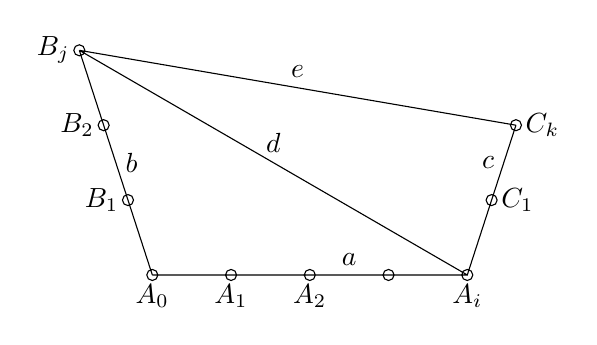
\begin{tikzpicture}
\begin{scope}[scale=1]
\begin{scope}
\draw[] (0,0) circle(2pt) node[below]{$A_i$}
-- ++(-1,0) circle(2pt)
-- node[above]{$a$} ++(-1,0) circle(2pt) node[below]{$A_2$}
-- ++(-1,0) circle(2pt) node[below]{$A_1$}
-- ++(-1,0) circle(2pt) node[below]{$A_0$}
-- ++(108:1) circle(2pt) node[left]{$B_1$}
-- node[right]{$b$} ++(108:1) circle(2pt) node[left]{$B_2$}
-- ++(108:1) circle(2pt) node[left]{$B_j$}
-- node[above]{$d$} (0,0)
-- ++(72:1) circle(2pt) node[right]{$C_1$}
-- node[left]{$c$} ++(72:1) circle(2pt) node[right]{$C_k$}
-- node[above]{$e$} ++(-5.545,0.951); % (-4-5*cos(72M),sin(72))
\end{scope}
\end{scope}
\end{tikzpicture}
\caption{Regular pentagon basic diagonals $d$ and $e$ from sides segments $a\ge\ b\ge c$.}
\label{fig:diagonals}
\end{figure}

From figure \ref{fig:diagonals} we know the regular internal pentagons angles equal $3\pi/5$:
\begin{align}
\alpha &= \angle{A_0A_iB_j} \\
\beta  &= \angle{B_jA_iC_k} \\
\theta &= \angle{B_jA_0A_i} \\
  &= \alpha + \beta \\
\cos\theta &= \frac{1-\sqrt{5}}{4}
\end{align}
From the law of cosines we calculate distance $d$ from integers $a,b$ which equal respectively to
iterators $i,j$:
\begin{align}
d &= \sqrt{a^2 + b^2 - 2ab\cos\theta} \nonumber\\
 &= \sqrt{a^2 + b^2 - 2ab\left(\frac{1-\sqrt{5}}{4}\right)} \nonumber\\
 &= \frac{\sqrt{4a^2 + 4b^2 - 2ab +2ab\sqrt{5}}}{2}
\end{align}
We define two integers $m, n$ to simplify last equation and obtain:
\begin{align}
m &= 4a^2 + 4b^2 - 2ab \\
n &= 2ab \\
d &= \frac{\sqrt{m + n\sqrt{5}}}{2}
\end{align}
\end{document}
